% Compile to an SVG with:
%
%     pdflatex tixz-learn.tex
%     inkscape -l tixz-learn.svg tixz-learn.pdf

\documentclass[crop,tikz]{standalone}
\usepackage{amsmath}

\begin{document}

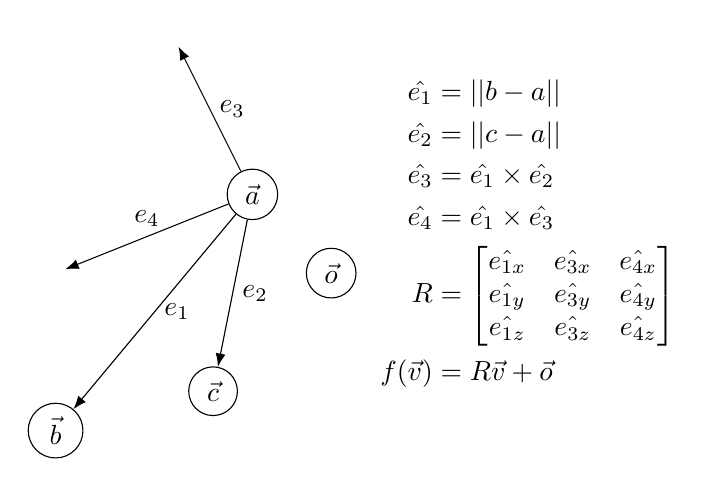
\begin{tikzpicture}[
		trianglenode/.style={
		% The shape:
		circle,
		% The size:
		minimum size=6mm,
		% The border:
		%very thick,
		draw=black,
		% The filling:
		top color=white,
		bottom color=white,
		% Font
		font=\itshape
    		}
	]
	% latex-latexnew, o-onenew, etc. arrows (see: https://tex.stackexchange.com/questions/5461/is-it-possible-to-change-the-size-of-an-arrowhead-in-tikz-pgf)
	\usetikzlibrary{arrows.meta}
	\usetikzlibrary{matrix}
	
	\node (A)[trianglenode] at (3.5,5) {$\vec{a}$};
	\node (B)[trianglenode] at (1,2)  {$\vec{b}$};
	\node (C)[trianglenode] at (3,2.5) {$\vec{c}$};
	\node (E3) at (2.5,7) {};
	\node (E4) at (1,4) {};
	\node (O)[trianglenode] at (4.5, 4) {$\vec{o}$};
	
	\node (EQN)[align=left] at (7,4.5) {$
		\begin{aligned}
			\hat{e_1} &= ||b-a||\\
			\hat{e_2} &= ||c-a||\\
			\hat{e_3} &= \hat{e_1} \times \hat{e_2}\\
			\hat{e_4} &= \hat{e_1} \times \hat{e_3}\\
			R &= \begin{bmatrix}
				\hat{e_{1x}} & \hat{e_{3x}} & \hat{e_{4x}} \\
				\hat{e_{1y}} & \hat{e_{3y}} & \hat{e_{4y}} \\
				\hat{e_{1z}} & \hat{e_{3z}} & \hat{e_{4z}} \end{bmatrix}\\
			f(\vec{v}) &= R\vec{v} + \vec{o}
		\end{aligned}
	$};

  	\draw [-Latex] (A) -- node[anchor=west]  {$e_1$} (B);
  	\draw [-Latex] (A) -- node[anchor=west]  {$e_2$} (C);
  	\draw [-Latex] (A) -- node[anchor=west]  {$e_3$} (E3);
  	\draw [-Latex] (A) -- node[anchor=south] {$e_4$} (E4);
\end{tikzpicture}
\end{document}